\section{Results}
\label{sec:results}

\subsection{Synthetic load}
Table~\ref{tab:synthetic} summarises the \texttt{stress-ng} tiers. Default Linux (A) missed deadlines in every loaded tier, up to 39.2\,\% of cycles under core-0 heavy load, and its worst case reached 18.0--27.9\,ms under all-core load. \texttt{SCHED\_FIFO} (B) held the deadline in every tier, although one run reached 973\us{}. B-iso stayed near 0.3\,ms under any stress. Config C with tuned priorities stayed at about 8\us{} at every tier, idle included: Linux load did not reach it.

\begin{table}[t]
\centering
\caption{Worst-case lateness under \texttt{stress-ng} (µs, mean of runs; DMR = highest miss ratio of any run)}
\label{tab:synthetic}
\small
\setlength{\tabcolsep}{3.5pt}
\resizebox{\columnwidth}{!}{%
\begin{tabular}{@{}lrrrrr@{}}
\toprule
Config & Idle & Core-0 med. & Core-0 heavy & All-core & DMR \\
\midrule
A & 545 & 5{,}304 & 6{,}321 & 21{,}580 & 39.2\,\% \\
B & 471 & 755 & 489 & 661 & 0 \\
B-iso & 96 & 324 & 329 & 324 & 0 \\
C, IPC stock & 759 & 795 & 809 & 759 & 0 \\
C, IPC tuned & 8.1 & 7.9 & 7.7 & 7.8 & 0 \\
\bottomrule
\end{tabular}}
\\[2pt]\footnotesize Source: \texttt{results/phase5d/compare\_configs.md}; 3 runs per cell (C all-core: 1).
\end{table}

\texttt{stress-ng} only creates busy programs, which a real-time thread preempts at once. The realistic loads below also make the kernel work.

\subsection{Realistic load}
Table~\ref{tab:realload} gives the worst cases and miss ratios under realistic load, and Fig.~\ref{fig:blocks} shows the worst case of every 10{,}000-cycle block. A's blocks sat at 4--15\,ms whenever the CNN ran. B stayed below 1\,ms under the CNN alone (\texttt{rdeploy}: 0 misses in 360{,}000 cycles) but crossed it once network traffic was added. B-iso exceeded 1\,ms in all 36 of its \texttt{rboth} blocks. Config C stayed between 6.3 and 10.5\us{} in every tier, idle included, with no misses.

\begin{table}[t]
\centering
\caption{Realistic load: worst case (range of 2 runs), typical block worst case, and misses over 1\,ms with 95\,\% interval}
\label{tab:realload}
\small
\setlength{\tabcolsep}{2.5pt}
\resizebox{\columnwidth}{!}{%
\begin{tabular}{@{}llrrl@{}}
\toprule
Config & Tier & WCL (ms) & Block (ms) & Misses (\%) \\
\midrule
A & rnet & 1.49--1.71 & 0.56 & 0.0022 (0.0011--0.0044) \\
A & rdeploy & 11.8--15.0 & 5.89 & 1.48 (1.45--1.52) \\
A & rboth & 8.36--10.7 & 5.61 & 3.54; runs 4.72, 2.36 \\
B & rnet & 0.99--1.16 & 0.73 & 0.0011 (0.0004--0.0029) \\
B & rdeploy & 0.52--0.55 & 0.14 & 0 ($\le$0.0008) \\
B & rboth & 1.45--1.54 & 0.31 & 0.025 (0.020--0.031) \\
B-iso & rnet & 0.76--0.82 & 0.52 & 0 ($\le$0.0008) \\
B-iso & rdeploy & 0.57--0.65 & 0.40 & 0 ($\le$0.0008) \\
B-iso & rboth & 1.59--1.72 & 1.46 & 0.23 (0.22--0.25) \\
C & idle & 0.0063--0.0070 & 0.0067 & 0 ($\le$0.015) \\
C & rnet & 0.0081--0.0083 & 0.0082 & 0 ($\le$0.015) \\
C & rdeploy & 0.0070--0.0082 & 0.0076 & 0 ($\le$0.015) \\
C & rboth & 0.0076--0.0105 & 0.0091 & 0 ($\le$0.015) \\
\bottomrule
\end{tabular}}
\\[2pt]\footnotesize Linux: 2 runs $\times$ 180{,}000 cycles; C: 2 runs $\times$ 10{,}000 cycles. Sources: \texttt{results/phase6b/realload.md}, \texttt{headline\_stats.md}.
\end{table}

\begin{figure}[t]
\centering
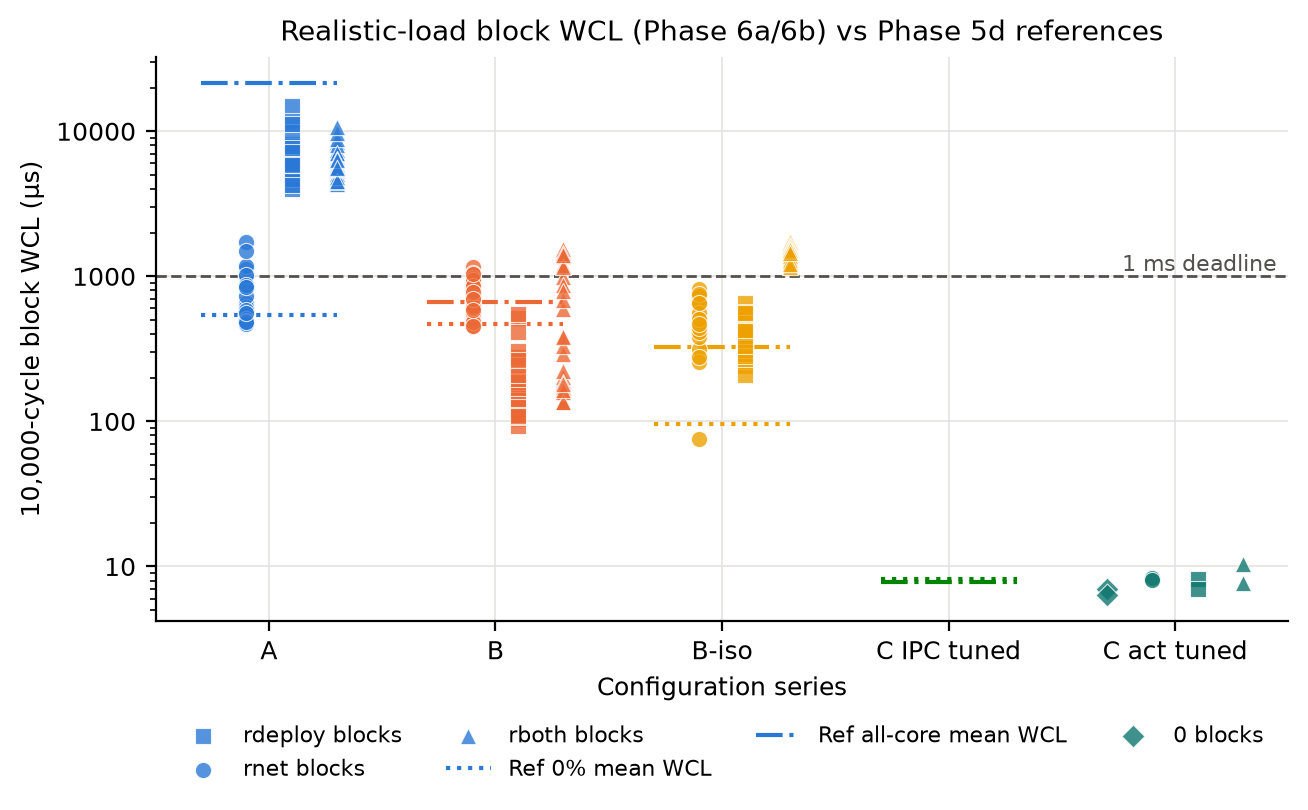
\includegraphics[width=\columnwidth]{block_wcl.png}
\caption{Worst-case lateness of every 10{,}000-cycle block under realistic load (log scale; dashed line: 1\,ms deadline). Config C stays near 10\us{} in every tier.}
\label{fig:blocks}
\end{figure}

Compared per block under \texttt{rboth}, Config C's typical worst case was 34$\times$ below B (plausible range 18--103$\times$, because B's blocks vary widely), 161$\times$ below B-iso (133--197$\times$) and 619$\times$ below A (528--797$\times$). The gap to B was smallest under the CNN alone, 19$\times$ (16--24$\times$), and largest under network traffic alone, 88$\times$ (82--98$\times$).

\subsection{Reserving a core made SCHED\_FIFO worse}
Under \texttt{rboth}, B-iso's worst case (1.59--1.72\,ms) and miss ratio (0.23\,\%) were worse than plain B's (1.45--1.54\,ms, 0.025\,\%). Fig.~\ref{fig:cpu3} shows the kernel work counted on core 3. Under \texttt{rboth} the ``reserved'' core received 654 function-call IPIs per second in B-iso against 60 in B, and about 440 against 220 softirqs per second. It was 24\,\% busy although none of our programs ran there; under the CNN alone it was only 4\,\% busy. Under \texttt{rnet} alone core 3 received \emph{less} kernel work in B-iso than in B, yet B-iso still exceeded the 0.5\,ms we predicted, so another mechanism, such as shared cache or memory traffic, may contribute.

\begin{figure}[t]
\centering
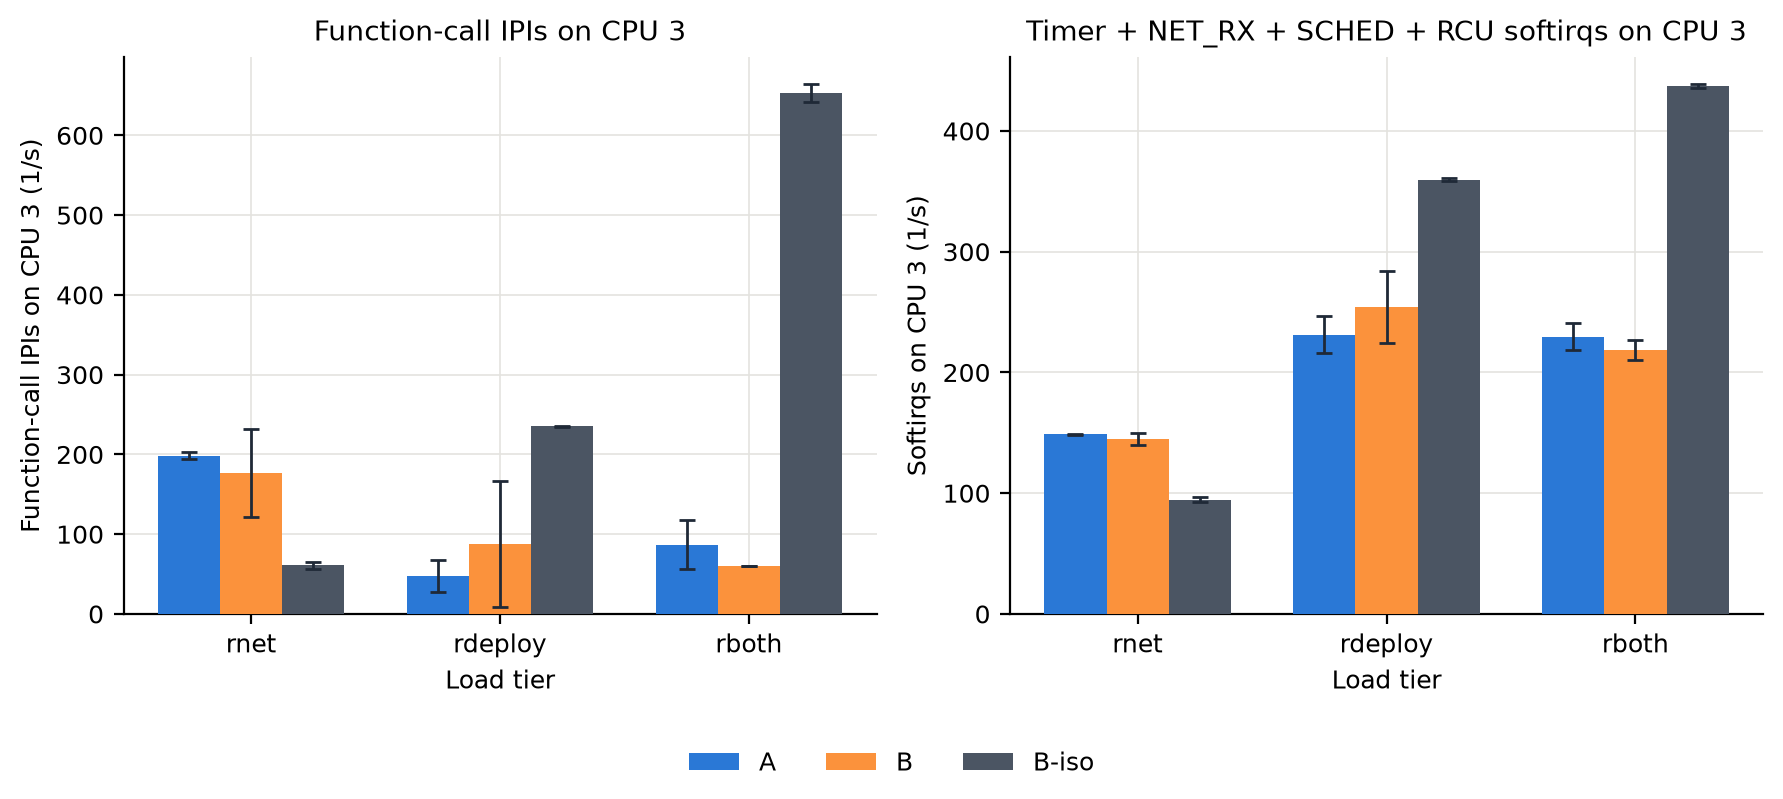
\includegraphics[width=\columnwidth]{cpu3_kernel_work.png}
\caption{Kernel work per second on CPU 3 for B and B-iso (run averages over 2 repeats).}
\label{fig:cpu3}
\end{figure}

\subsection{On the microcontroller, priority decided the result}
Table~\ref{tab:mcu} compares the four Config C variants under \texttt{stress-ng}. With library defaults, adding the link raised the worst case from 20--41\us{} to 759--809\us{}, already at idle. In the stock IPC runs, 72--83\,\% of the late cycles (over 100\us) contained a setpoint arrival, against a base rate of 11.7\,\%. Raising the loop above the bridge thread brought the IPC worst case to 7.7--8.1\us{} and the number of such late cycles from 84--121 per run to zero. The tuned link still costs about 6\us{} over the tuned baseline.

\begin{table}[t]
\centering
\caption{Config C variants under \texttt{stress-ng}: worst case (µs), range of tier means}
\label{tab:mcu}
\small
\begin{tabular}{@{}lll@{}}
\toprule
Variant & Loop priority & Worst case \\
\midrule
Stock, no IPC & below bridge (14 vs 5) & 20--41 \\
Stock, with IPC & below bridge & 759--809 \\
Tuned, no IPC & above bridge (4 vs 5) & 1.5--1.7 \\
Tuned, with IPC & above bridge & 7.7--8.1 \\
\bottomrule
\end{tabular}
\\[2pt]\footnotesize 3--4 runs per tier. Source: \texttt{results/phase5d/compare\_configs.md}, \texttt{ipc\_attribution.md}.
\end{table}

\subsection{The full chain to the drive}
In eight Config C runs (idle and the three realistic tiers, two each), all 1{,}920 speed commands reached the drive emulator with the right value: none lost, wrong or duplicated. The drive saw each new command 1.47--4.11\,ms after the tick that applied it, and this delay was the same at idle and under every load, because it is set by the 500\,Hz PWM (waiting for the next period plus the pulse width), not by Linux. Linux load only stretched the time a setpoint took to reach the MCU: the 99th-percentile round trip grew from 12.8\,ms at idle to 15.7\,ms under \texttt{rboth}. The loop never waited for it.

\subsection{Predictions}
Of the 15 predictions written before the realistic and full-chain runs, 12 held, one held partly and two failed. A's miss ratio under \texttt{rdeploy} exceeded the predicted 1\,\% (1.42--1.55\,\%). B-iso under \texttt{rnet} stayed above 0.5\,ms although the Wi-Fi interrupt had been moved off core 3. The setpoint round trip under \texttt{rnet} was not longer than at idle: the sender suffers from CPU contention, not from network interrupts.
